\documentclass{VUMIFPSbakalaurinis}
\usepackage{float}
\usepackage{hyperref}
\usepackage{algorithmicx}
\usepackage{algorithm}
\usepackage{algpseudocode}
\usepackage{amsfonts}
\usepackage{amsmath}
\usepackage{bm}
\usepackage{caption}
\usepackage{color}
\usepackage{graphicx}
\usepackage{listings}
\usepackage{subcaption}
\usepackage{wrapfig}
\usepackage{biblatex}
\usepackage{microtype}
\usepackage{mathtools}


% Titulinio aprašas
\university{Vilniaus universitetss}
\faculty{Matematikos ir informatikos fakultetas}
\institute{Informatikos institutas}  % Užkomentavus šią eilutę - institutas neįtraukiamas į titulinį
\department{Programų sistemų bakalauro studijų programa}
\papertype{Laboratorinio darbo ataskaita}
\title{Dirbtinio neurono modelis}
\titleineng{Artificial Neuron Model}
\author{Armintas Pakenis}
% \secondauthor{Vardonis Pavardonis}   % Pridėti antrą autorių
\supervisor{prof. dr. Olga Kurasova}
\reviewer{prof. dr. Olga Kurasova}
% \addsignatureplaces{} % prideda parašų vietas tituliniame puslapyje
\date{Vilnius – \the\year}

\bibliography{bibliografija}

\begin{document}
\maketitle

%% Padėkų skyrius
% \sectionnonumnocontent{}
% \vspace{7cm}
% \begin{center}
%     Padėkos asmenims ir/ar organizacijoms
% \end{center}

\tableofcontents

\section{Užduoties tikslas}
Užduoties tikslas – suprasti dirbtinio neurono modelį, 
jo veikimo principus, rasti svorius, 
kuriuos neuronas naudodamas gautų tinkamas išvestis. 
Naudotos pradinės įvestys ir išvestys pateiktos \ref{tab:duomenys}
lentelėje. Programos kodas rašytas Jupyter
užrašų knygutės aplinkoje, jį rasti galima GitHub repositorijoje: 
\href{https://github.com/ArmintasP/Computational-intelligence/tree/main/Lab1}{\color{cyan}{https://github.com/ArmintasP/Computational-intelligence/tree/main/Lab1}}.

% tablesgenerator.com - converts calculators (e.g. excel) tables to LaTeX
\begin{table}[H]\footnotesize
  \centering
  \caption{Klasifikavimo duomenys ir klasės}
  {\begin{tabular}{|cc|c|ll}
    \cline{1-3}
    \multicolumn{2}{|c|}{Duomenys}    & Klasė &  &  \\ \cline{1-3}
    \multicolumn{1}{|c|}{$x_1$} & $x_2$ & $t$     &  &  \\ \cline{1-3}
    \multicolumn{1}{|c|}{–0,3} & 0,6  & 0     &  &  \\ \cline{1-3}
    \multicolumn{1}{|c|}{0,3}  & –0,6 & 0     &  &  \\ \cline{1-3}
    \multicolumn{1}{|c|}{1,2}  & –1,2 & 1     &  &  \\ \cline{1-3}
    \multicolumn{1}{|c|}{1,2}  & 1,2  & 1     &  &  \\ \cline{1-3}
    \end{tabular}}
  \label{tab:duomenys}
\end{table}


\section{Svorių ieškojimo strategija}
Buvo ieškoma svorių $w_0$, $w_1$, $w_2$, kur $w_0$ – poslinkis,
o $x_0 = 1$. Šių svorių rinkinys buvo sudaromas
kiekvienam svorio kintamajam priskiriant
pseudoatsitiktinio skaičiaus reikšmę iš intervalo $[-a; a]$,
 kur $a$ buvo pasirinktas
$7$. Jei su svorių rinkiniu naudojant pasirinktą
 aktyvacijos funkciją buvo gaunama norima išvestis
 (žr. į lentelės \ref{tab:duomenys} $t$ reikšmes), laikoma,
 kad svoriai rasti. Jei ne, rinkinys generuojamas iš naujo,
 kol randami tinkamas prognozes duodantys svoriai.

\subsection{Svorių ieškojimo sprendimas grafiniu būdu}

Svorius galima rasti ne tik programos pagalba, bet ir grafiniu
būdu išsprendžiant šią nelygybių sistemą, 
kai aktyvacijos funkcija slenkstinė:

\begin{equation*}
  \begin{dcases}
    w_0 - 0,3w_1 + 0,6w_2 < 0 \\
    w_0 + 0,3w_1 - 0,6w_2 < 0 \\
    w_0 + 1,2w_1 - 1,2w_2 \geq  0 \\
    w_0 + 1,2w_1 + 1,2w_2 \geq  0
  \end{dcases}
\end{equation*}

\ref{img:visi-sprendiniai} pav. pateiktas grafinis
nelygybių sistemos sprendimas, kai visi sprendiniai
privalo būti intervale $[-7, 7]$.
Galima pastebėti, kad kai poslinkis bus teigiamas ar lygus 0,
sprendiniai neegzistuos.
Rasti konkrečius sprendinius iš grafiko gali būti paprasčiau,
jei poslinkio reikšmę fiksuosime.
Tarkime, kad $w_0 = -1$. Tuomet $w_1$ ir $w_2$ galima bus lengviau
parinkti iš grafiko (žr. \ref{img:dalinis} pav.).

% \begin{figure}[H]
%     \centering
%     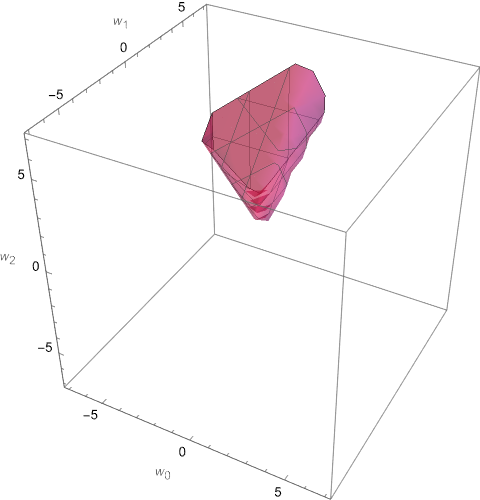
\includegraphics[scale=0.5]{img/3d-2.png}
%     \caption{Grafinis sprendinių atvaizdavimas}
%     \label{img:visi-sprendiniai}
% \end{figure}

% \begin{figure}[H]
%   \centering
%   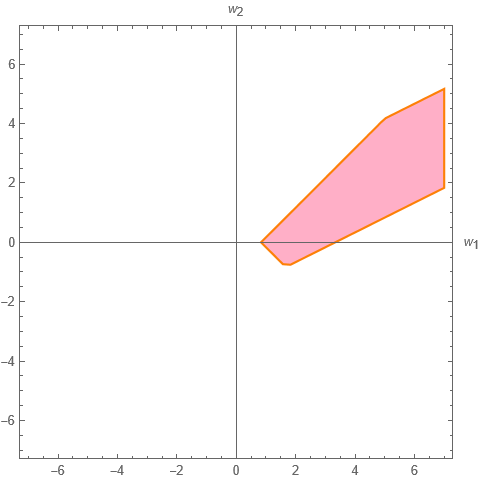
\includegraphics[scale=0.5]{img/minus1.png}
%   \caption{Grafinis sprendinių atvaizdavimas, kai $w_0 = -1$}
%   \label{img:dalinis}
% \end{figure}

\begin{figure}[H]
  \begin{minipage}[c]{0.4\linewidth}
    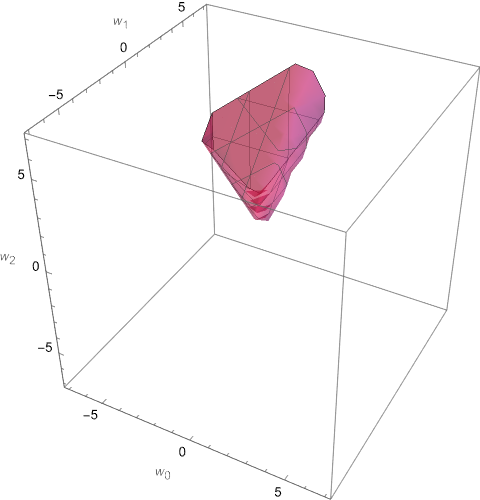
\includegraphics[scale=0.5]{img/3d-2.png}
    \caption{Grafinis sprendinių atvaizdavimas}
    \label{img:visi-sprendiniai}
  \end{minipage}
  \hfill
  \begin{minipage}[c]{0.4\linewidth}
    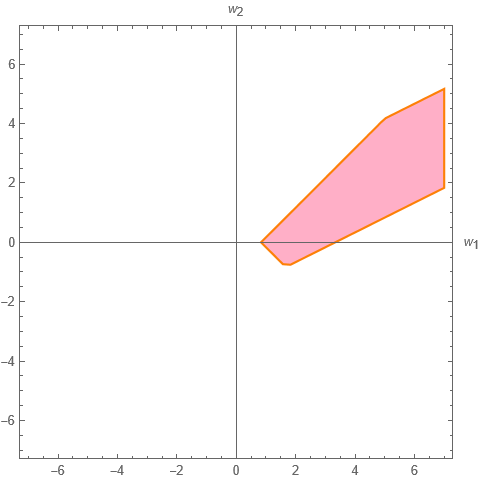
\includegraphics[scale=0.5]{img/minus1.png}
    \caption{Grafinis sprendinių atvaizdavimas, kai $w_0 = -1$}
    \label{img:dalinis}
  \end{minipage}%
\end{figure}


Akivaizdu, kad $w_0 = -1$, $w_1 = 4$, $w_2 = 2$ kartu
yra lygybės sprendiniai; tuo galima įsitikinti jų reikšmes
įstačius į nelygybių sistemą:
\begin{equation*}
  \begin{dcases}
    w_0 - 0,3w_1 + 0,6w_2 = -1 - 0,3 \cdot 4 + 0,6 \cdot 2 = -1 - 1,2 + 1,2 = -1  < 0 \\
    w_0 + 0,3w_1 - 0,6w_2 = -1 + 0,3 \cdot 4 - 0,6 \cdot 2 = -1 + 1,2 - 1,2 = -1< 0 \\
    w_0 + 1,2w_1 - 1,2w_2 = -1 + 1,2 \cdot 4 - 1,2 \cdot 2 = -1 + 4,8 - 2,4 = 1,4 \geq  0 \\
    w_0 + 1,2w_1 + 1,2w_2 = -1 + 1,2 \cdot 4 - 1,2 \cdot 2 = -1 + 4,8 + 2,4 = 6,4 \geq  0
  \end{dcases}
\end{equation*}

\section{Programos rezultatai}
Šio skyriaus poskyriuose pateikiamos programos apskaičiuotos
svorių reikšmės naudojant skirtingas aktyvacijos funkcijas.

Reikšmės pateikiamos poziciškai, pvz.: $
\begin{bmatrix}
  0 & 1 & 2
\end{bmatrix}
$ atitiks
$w_0 = 0$, $w_1 = 1$, $w_2 = 2$.

\subsection{Svoriai gauti naudojant slenkstinę aktyvacijos funkciją}
Sprendiniai:$
\begin{bmatrix}
  -6,64 & 6,02 & -0,37
\end{bmatrix},
\begin{bmatrix}
  -0,29 & 2,15 & 1,48
\end{bmatrix},
\begin{bmatrix}
  -3,05 & 5,69 & 2,94
\end{bmatrix}.
$

\subsection{Svoriai gauti naudojant sigmoidinę aktyvacijos funkciją}
Sprendiniai:$
\begin{bmatrix}
  -2,7 & 5,31 & 1,71
\end{bmatrix},
\begin{bmatrix}
  -4,49 & 6,93 & 1,53
\end{bmatrix},
\begin{bmatrix}
  -0,86 & 5,32 & 3,08
\end{bmatrix}.
$

\end{document}
